\documentclass[11pt]{article}

\usepackage{epsf}
\usepackage{epsfig}
\usepackage{url}
\usepackage{6829hw}
\input{macros.tex}

\begin{document}

\newcounter{listcount}
\newcounter{sublistcount}


\handout{H1}{February 27, 2013}{Instructor: Prof. Nick Feamster}
{College of Computing, Georgia Tech}{Problem Set 2: Routing and
  Transport Layer} 

%This problem set has three questions, each with several parts.  Answer
%them as clearly and concisely as possible.  You may discuss ideas with
%others in the class, but your solutions and presentation must be your
%own.  Do not look at anyone else's solutions or copy them from
%anywhere. (Please refer to the Georgia Tech honor code, posted on the
%course Web site).

Turn in your writeup and talk on {\bf March 15, 2013} by 11:59pm.
{\em Please upload your solutions to T-Square.  Other forms of
  submission will not be accepted!}  We will be providing more
information about how to turn in your assignment as the due date
approaches.


\section{BGP Routing Policies}

Consider the figure below, which shows a set of ASes and different
peering and customer-provider relationships, as we learned about in
class. Each arrow shows the direction from customer to provider (i.e.,
the flow of money).  Assume that all customer-provider relationships are
the same price.  Also, assume that all ASes follow the preference and
export rules that we discussed in class.

\begin{center}
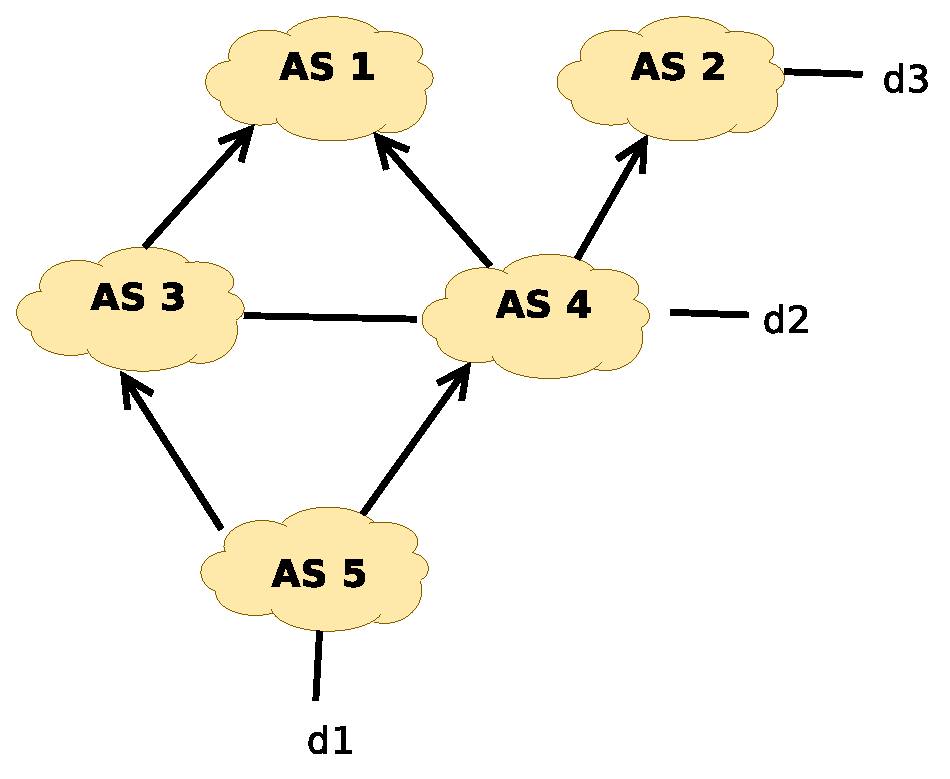
\includegraphics[width=3in]{as-rel}
\end{center}

\begin{enumerate}
\item Which path will AS~2 choose to reach AS~7?  Why?
\item Will AS~1 be able to use AS~4 to reach AS~2?  Why or why not?
\item This graph actually has a partition (i.e., two ASes that will not
  learn routes about each other's customers).  Explain which two ASes
  are partitioned from one another and why the partition exists.
\end{enumerate}

\section{Socket Programming}

This problem will give you practice with socket programming.  There are
two parts to the assignment: 
\begin{enumerate}
\itemsep=-1pt
\item Write a client and server using TCP to transfer an arbitrary size
  binary file across a network.
\item Write a client and server using UDP to transfer an arbitrary size
  binary file across a network.
\item You can chose to do one of the following:
\begin{itemize}
\itemsep=-1pt
 \item Write Python client code that performs a TCP transfer across the
   network.  The server must be written in C (You can use your code from
   part~1).
\item Write C client code to implement your own reliability scheme for
  UDP protocol transfer. The UDP file transfer should end up
  recovery the whole file at the server. 
\end{itemize}
\end{enumerate}

{\bf Deliverables:}
You shoud submit your code in the following heirarchy :
Part 1, Part 2, Part 3 folders with each containing src/, bin/ ,doc/ ,
include/ folder.
\begin{itemize}
\itemsep=-1pt
\item src must have your code
\item bin must have your own binary file
\item doc must have documentation of how to run and test your code
\item include must have the header files
\item Have a Makefile
\end{itemize}

{\bf Graphs expected:}
\begin{enumerate}
\itemsep=-1pt
\item You should run each of Part 1, Part 2, Part 3 of your code
  with client code on your laptop and Server code on any of the Gatech
  servers.  Transfer files of the following sizes: 1 KB, 5 KB, 50 KB,
  100 KB, 1 MB, 10 MB, 100 MB, 1 GB.  {\em Perform each of these
    transfers five times and record the times taken for each transfer.}
\item Calculate the mean and standard deviation of the five observation.
\item Plot the graph of time taken for each file transfer across the
  network.  The x axis of your graph should be file size, and the y axis
  should be the average time taken to transfer a file of that size.
\item Give any other interesting observations.  You can submit one graph
  with three separate lines, one for each pf Parts 1, 2, and 3.
\end{enumerate}


\section{Domain Name System}


In this question, you will perform some hands-on DNS queries using {\tt
  dig} and play with DNS lookups from various applications to understand
more about the DNS.  In the second part of this question, you will
implement a variation on a stub DNS resolver.

RFC~1035 may be helpful for answering some of these questions.  


\begin{enumerate}
\item We'll first warm up by learning a few things about Georgia Tech's
  DNS setup.  You may find {\tt dig} helpful for completing this
  problem. Run ``{\tt traceroute ai}'' from some machine on the Georgia
  Tech campus network. (Depending on where on the campus you run this
  experiment, you may see different results.  If this isn't producing
  anything interesting for you, look at the ``hostname'' entry in your
  /etc/hosts file and explain what it does and what you're seeing when
  you run the above command.) Now run ``{\tt traceroute ai.}'' from the
  same machine.  Include the output from each run in your problem set
  writeup.  Are the two traceroutes running traces to different
  machines?  Why or why not?

\item What are the authoritative nameservers for {\tt gatech.edu}?  How
  long will your resolver cache the records pointing to these
  nameservers?  

  What are the College of Computing's authoritative nameservers (\ie, for
  the domain {\tt cc.gatech.edu})?  Give two benefits of topologically
  diverse authoritative nameservers.

  Why do NS records return names, rather than IP addresses?

\item What is another ``canonical name'' for the College of Computing's
  Web server?  

\item What is are the mail exchanges for {\tt cc.gatech.edu}?
\end{enumerate}


\section{Back-of-the-Envelope Calculations for Networking}

Perform some quick back-of-the-envelope calculations for the following
values.  {\em These questions are intentionally vague.  Show your work.}
\begin{enumerate}
\item What is the expected round-trip time for a packet between San
  Francisco and New York, assuming no queueing delay. (Assume speed of
  light propagation.)
\item How much memory would a typical Internet routing table require?
  Hint: Find out how many IP prefixes are in a routing table.  Then,
  estimate how large each routing table entry must be.
\item How long does a DNS lookup typically take on a cache hit, assuming
  initial lookups to a local resolver on the LAN?  How long would it likely take
  if the A record were not in the local cache?  How long would it take
  if the NS record for the second-level domain were not in the local
  cache?
\item Suppose that the MTU for an IP packet on a Gigabit Ethernet network is
  increased from 1500 bytes to 9000 bytes.  How does this affect the
  likelihood of collision?  How does it affect efficiency?  Try to be as
  specific as you can.
\end{enumerate}


\section{BGP Routing Table Dumps}

For this question, you will need to download the Routeviews routing
table from
\url{http://www.gtnoise.net/classes/cs3251/spring_2013/psets/ps2//tmp/rib.20130227.2000.txt.gz}
This file contains a Cisco BGP4 routing table snapshot, taken at Oregon
Route Views (\url{http://www.routeviews.org/}) on February 27,
2013. ({\em Beware:} This is a text file that is 50+ MB, compressed.
You should be able to analyze it without uncompressing it using, for
example {\tt zcat}.  Do NOT try to open it in a text editor, or you will
be sorely disappointed.)

If you are curious about what other snapshots look like, you
can find daily snapshots at \url{http://archive.routeviews.org/}


\begin{enumerate}

\item Find the routing table entry for the Georgia Tech
  campus network.

\setcounter{listcount}{0}
\begin{list}{(\alph{listcount})}{\usecounter{listcount}}

\item What is the IP address of the best next hop from this router to
Georgia Tech?  How does this router know how to reach that next hop IP
address?

\item What is the AS number for Georgia Tech? 

\item What are all of the IP prefixes that Georgia Tech advertises to
  this router?  Why does Georgia Tech advertise more than one prefix?

\item Give an example of two IP prefixes that Georgia Tech advertises
  that ``overlap'' in IP address space.  What is the reason that Georgia
  Tech would advertise two routes for overlapping IP address space?

\item Give the sequence of ASes that Sprint (AS~1239) would likely take
  to {\tt 130.207.0.0/16}?  To {\tt 128.61.64.0/18}?  Given that these
  prefixes both belong to Georgia Tech, why would the AS paths differ?

\item How many routes are there to get from this router to Georgia Tech?

\item How many ASes must a packet traverse between the time it
leaves the router and the time that it arrives at Georgia Tech, for each
of the routes?  What would determine which route is the ``best'' route,
in each case?

\item What are the AS numbers of all of Georgia Tech's upstream
  providers? What ISP does the above AS correspond to?  ({\em Hint:} You
  can discover this information using a whois query.)

\item In paths where Georgia Tech uses Cogent (AS~174) as an upstream,
  the AS path ends with five instances of the same AS number.  Why?
  What is the likely relationship between this AS number and Cogent?

\item Look at all of the routes for which the AS path contains the
  sequence {\tt 11537 10490}.  What do the ASes that appear first in
  those AS paths all have in common?  Why wouldn't the ASes that select
  paths that don't have {\tt 11537 10490} in them not be selecting those
  paths? 

\item Use {\tt traceroute} to measure route from some machine at Georgia
  Tech to {\tt archive.routeviews.org}.  Please include the output
  of your traceroute with your problem set.

  Find the sequence of ASes that correspond to this traceroute.  {\em
    Hint:} You can do this either with a special version of traceroute,
  or you can manually look up the IP addresses with whois.  Some
  versions of traceroute such as ``nanog traceroute'' will do the AS
  lookups for you automatically.

  Is the sequence of ASes from Georgia Tech to the router the same as the
  reverse route in the trace data?   Why might the reverse path differ?
  (Please list reasons other than the fact that your traceroute was
  performed at a different time as the table snapshot!)
\end{list}

\item Find an example routing table entry where the AS number on the AS
  path is repeated more than once.  Explain what this behavior is.
  Which AS likely caused the AS number to appear multiple times, and
  why?  (We discussed this in class.)

\item Write a script to count the number of entries in the routing table
  that have prefixes of different lengths.  What is the most common
  prefix lengths?  Explain the tradeoffs between longer and shorter
  prefix lengnths.

\end{enumerate}

\pagebreak
\section{Book Problems}

Please complete the following problems from Kurose and Ross, 6th
Edition:

\noindent
{\bf Chapter 4.}
\begin{enumerate}
\itemsep=-1pt
\item {\em Head of Line Blocking.} P9
\item {\em Link-State Routing.} P26
\item {\em Count to Infinity.} P34
\end{enumerate}



\end{document}
